\Chapter{Keresztfordítás}

\section{Formális nyelvek}

A programozási nyelvek formális nyelvek.

\subsection{Véges automaták}


\subsection{Reguláris nyelvek}

A reguláris nyelvek a véges automatákkal leírható nyelvek.

% TODO: EBNF jelölésrendszere

% TODO: Railroad/szintaxis diagramok (Pl.: JSON.org, SQLite dokumentáció)

\section{A feldolgozás lépései}

Leírni a fordítás lépéseit. Ehhez rögtön az elején lehet egy ábra, amit aztán külön pontok részleteznek.

Meg kell indokolni (röviden), hogy miért az említett nyelvek kerültek kiválasztásra.

Az esetleges nehézségekre, kihívásokra már itt fel lehet hívni a figyelmet.

A feldolgozás lépéseinek áttekintését láthatjuk \aref{fig:process}. ábrán.

\begin{figure}
\centering
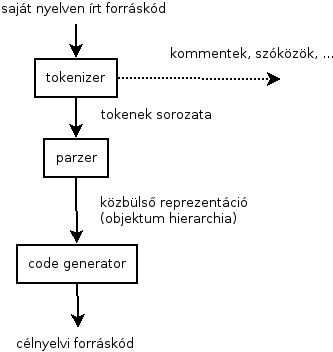
\includegraphics[scale=1]{kepek/process.png}
\caption{A keresztfordítás lépései}
\label{fig:process}
\end{figure}

\section{Tokenizálás}

% TODO: Parser-tokenizer (lexer) kapcsán írni néhány dolgot áttekintés képpen.

% TODO: Gyakori tokenek (szám-, szöveg literál, operátorok, zárójelek, kommentek, szóközök és egyéb fehér karakterek)
